\documentclass[a4paper]{article}

% Linguagem
\usepackage[utf8]{inputenc}
\usepackage[portuguese]{babel}
\usepackage[T1]{fontenc}

% Pacotes matemáticos
\usepackage{amsmath}
\usepackage{amsfonts}
\usepackage{amssymb}
\usepackage{graphicx}

% Fontes e identaçãp
\usepackage{setspace}                   % espaçamento flexível
\usepackage{indentfirst}                % indentação do primeiro parágrafo
\usepackage[fixlanguage]{babelbib}
\usepackage[font=small,format=plain,labelfont=bf,up,textfont=it,up]{caption}

% Pacotes para cores e modelos
\usepackage[a4paper,top=3.0cm,bottom=2.0cm,left=3.0cm,right=2.0cm]{geometry} \usepackage[usenames,svgnames,dvipsnames]{xcolor}
\usepackage[pdftex,plainpages=false,pdfpagelabels,pagebackref,
            colorlinks=true,citecolor=DarkGreen,linkcolor=DarkRed,
            urlcolor=DarkRed,filecolor=DarkGreen,
            bookmarksopen=true]{hyperref}

% Pacote para imagens
\usepackage{graphicx}

% Novo nome para sumário
\renewcommand{\contentsname}{Sumário}

% Pacotes para itens
\usepackage{calc}  
\usepackage{enumitem}  

\title  {Métodos Formais e Lógica de Programação - EP1: Sudoku}
\author {Renato Cordeiro Ferreira}
\date   {}

%%%%%%%%%%%%%%%%%%%%%%%%%%%%%%%%%%%%%%%%%%%%%%%%%%%%%%%%%%%%%%%%%%%%%%%%%%%%%%%
\begin{document}

\maketitle

\tableofcontents

\newpage %%%%%%%%%%%%%%%%%%%%%%%%%%%%%%%%%%%%%%%%%%%%%%%%%%%%%%%%%%%%%%%%%%%%%%
\section{Introdução}
\label{sec:introducao}

  \subsection{Sudoku}
    O Sudoku é um jogo que consiste em completar números em um \emph{grid} 
    de tamanho 9x9 seguindo as seguintes regras:
    \begin{itemize}
      \item Em cada linha, deve aparecer apenas um número de 1 a 9;
      \item Em cada coluna, deve aparecer apenas um número no mesmo intervalo;
      \item O mesmo vale para cada \emph{subgrid}, de tamanhos 3x3. 
    \end{itemize}
  
  \subsection{Projeto}
    Este exercício consiste em criar um resolvedor de Sudokus, utilizando
    para isso a criação de \textbf{fórmulas} da Lógica Proposicional Clássica,
    na Forma Normal Conjuntiva. Estas fórmulas são, então, processadas pelo
    \emph{SAT solver} (resolvedor de satisfatibilidade). Por fim, a resposta
    é apresentada em forma de um Sudoku em ASCII.
  
  \subsection{Estrutura}
  
    Para informações sobre o uso de programa e os seus desenvolvedores,
    consultar os arquivos \href{run:../README.md}{\texttt{README.md}} e
    \href{run:../LICENSE}{\texttt{LICENSE}}. Também é possível usar a 
    opção \textbf{-h} no programa para exibir a ajuda.
  
    O programa consiste dos seguintes diretórios, que contém os arquivos 
    utilizados na implementação do projeto:
   
    \begin{itemize}
      \item \textbf{bin:}  Arquivo executáve principal do programa, além
                           de programas auxiliares individuais;
      \item \textbf{doc:}  Pasta para a documentação, com este arquivo, 
                           a versão fonte em \LaTeX, e a ajuda do programa
                           principal (em formatos \textbf{.txt} e de manual);
      \item \textbf{lib:}  Arquivos com classes/pacotes de Perl no formato
                           \texttt{.pm} e arquivos em C para compilação do
                           \emph{SAT solver};
      \item \textbf{test:} Arquivos de teste com entradas de Sudokus, em
                           formato \textbf{.txt}.
    \end{itemize}
    
\newpage %%%%%%%%%%%%%%%%%%%%%%%%%%%%%%%%%%%%%%%%%%%%%%%%%%%%%%%%%%%%%%%%%%%%%%

\section{sudoku}
\label{sec:sudoku}

  O programa principal para resolver os sudokus consiste de uma interface
  com o usuário para receber a condição inicial do Sudoku e resolvê-lo. 
  \ref{sec:bibliotecas}), para resolver o Sudoku dado como entrada.
  
  Nas seções abaixo, são descritas as funcionalidades do programa.
  Para detalhes sobre a implementação, ver seção \ref{sec:bibliotecas}.
    
  \subsection{Instalação}
  \label{subsec:instalacao}
  
    O programa \textbf{sudoku} é necessário o interpretador \emph{Perl},
    na versão 5.14 ou superior.
    
    Internamente, o programa usa um \emph{SAT solver} (resolvedor de 
    satisfatibilidade) para o cálculo. Por padrão, o resolvedor 
    \textbf{minisat} vem incluído com o código-fonte. Para compilá-lo,
    basta entrar no terminal e digitar, na pasta do projeto \texttt{make}.
    
    Para utilizar o resolvedor \textbf{zChaff} ou o \textbf{minisat}
    disponível em seu sistema, consultar a seção \ref{subsec:uso}.
  
  \subsection{Uso}
  \label{subsec:uso}
    
    O uso padrão do programa, por meio de linha de comando, é: 
    \begin{center}
    \textbf{sudoku} [-h] [-s] [-c] [-m|-z] [-p] \emph{entrada.txt}
    \end{center}
    
    Estão disponíveis as seguintes opções:
    \begin{itemize}
      
      \item \textbf{\texttt{-c, -{}-cnf-only}:} \\
        Não imprime a saída. Apenas gera o arquivo \textbf{.cnf} com as
        fórmulas para o \emph{SAT solver}.
        
      \item \textbf{\texttt{-h, -{}-help}:} \\
        Exibe a ajuda, em formato de manual ou \textbf{.txt}, se o 
        programa \emph{man} não estiver disponível no sistema.
        
      \item \textbf{\texttt{-m, -{}-minisat=\underline{s}}:} \\
        Configura o \emph{SAT solver} como sendo \textbf{minisat} (o
        resolvedor padrão), mas com um \emph{path} configurável para o
        executável do programa.
        
      \item \textbf{\texttt{-s, -{}-size=\underline{i}}:} \\
        Permite configurar o tamanho do Sudoku. Por padrão, é 9x9. 
        Esta opção recebe como argumento \textbf{obrigatório} um 
        inteiro que deve ser quadrado perfeito. Caso o número não
        seja neste formato, o comportamento do programa é indefinido.
        
      \item \textbf{\texttt{-p, -{}-proof}:} \\
        Cria um arquivo do tipo \textbf{.stat} com as estatísticas 
        geradas pelo \emph{SAT solver}.
        
      \item \textbf{\texttt{-s, -{}-size=\underline{i}}:} \\
        Configura um número quadrado perfeito (4, 9, 16, ...) como 
        sendo o tamanho do Sudoku (para jogos 4x4, 9x9, etc).
        
      \item \textbf{\texttt{-z, -{}-zchaff=\underline{s}}:} \\
        Configura o \emph{SAT solver} como sendo \textbf{zChaff} 
        (no lugar do \emph{minisat}). Recebe como argumento um 
        \emph{path} para o binário do programa (que \textbf{deve}
        se chamar "zchaff").
        
    \end{itemize}
    
    A saída padrão do programa é um Sudoku colorido, com os separadores
    de \emph{subgrids} em amarelo e os números da entrada em vermelho:
    
    \bigskip
    \begin{figure}[ht!] 
      \centering
      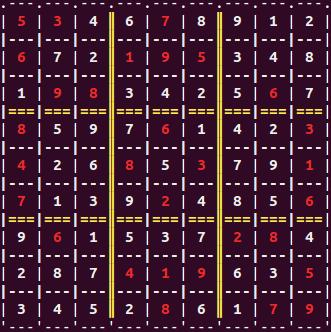
\includegraphics[width=70mm]{Sudoku.png}
      \caption{Exemplo de Sudoku impresso por padrão pelo programa} 
      \label{fig:sudoku}
    \end{figure}
    
  \subsection{Entrada}
  \label{subsec:entrada}
    
    A entrada do programa consiste de um arquivo no formato \textbf{.txt},
    com números separados por espaços representando o número naquela 
    posição dentro do jogo. 
    
    Para um Sudoku de ordem 9x9, um exemplo de entrada seria:
    
    \bigskip
    \texttt
    {
        5 3 0 0 7 0 0 0 0 6 0 0 1 9 5 0 0 0 0 9 8 0 0 0 0 6 0 8 0 0 0 6 0 0 
        0 3 4 0 0 8 0 3 0 0 1 7 0 0 0 2 0 0 0 6 0 6 0 0 0 0 2 8 0 0 0 0 4 1 
        9 0 0 5 0 0 0 0 8 0 0 7 9
    }
    \bigskip
    
    No qual estão dipostos 81 números de 0 a 9. Para a i-ésima posição do
    Sudoku, contando a partir do canto superior-esquerdo, o número colocado
    deve ser:
    \begin{itemize}
      \item de 1 a 9, se o número estiver apresentado no Sudoku inicial;
      \item 0, caso a posição no Sudoku esteja vazia.
    \end{itemize}
    
    Para sudokus de ordens maiores ou menores (16x16, 4x4, etc), a mesma
    regra vale, alterando-se apenas o intervalo de números (de 1 até o 
    número de linhas do Sudoku). A ordem do Sudoku é, por padrão, 9, e 
    pode ser redefinida conforme explicado pela seção \ref{subsec:uso}.
    
    Se no arquivo houver mais ou menos de $n^2$ variáveis, com $n$ a 
    ordem do Sudoku, o programa lança uma exceção correspondente.
    
    Alternativamente, para facilitar a visualização, o programa 
    \textbf{sudoku} aceita também entradas com quebras de linhas, 
    e com comentários iniciados por \texttt{\#}. Caso um comentário 
    seja colocado, tudo desde \texttt{\#} até o final da linha é ignorado. 
    
    \begin{center}
    \texttt
    {
        \# Meu exemplo de Sudoku \\
        5 3 0 0 7 0 0 0 0 \\
        6 0 0 1 9 5 0 0 0 \\
        0 9 8 0 0 0 0 6 0 \\
        8 0 0 0 6 0 0 0 3 \\
        4 0 0 8 0 3 0 0 1 \\
        7 0 0 0 2 0 0 0 6 \\
        0 6 0 0 0 0 2 8 0 \\
        0 0 0 4 1 9 0 0 5 \\
        0 0 0 0 8 0 0 7 9 
    }
    \end{center}
    
  \subsection{Saida}
  \label{subsec:saida}
  
    A saída padrão, feita pelo programa, é um Sudoku colorido, com os
    números da entrada em \textcolor{red}{vermelho}, e os separadores 
    de cada \emph{subgrid} em \textcolor{Goldenrod}{amarelo}, conforme 
    mostrado na Figura \ref{fig:sudoku}.
    
    Alternativamente, caso um arquivo com a resposta do \textbf{minisat}
    seja disponibilizada, o programa \textbf{draw\_sudoku.pl} imprime um
    Sudoku de forma mais legível.

\newpage %%%%%%%%%%%%%%%%%%%%%%%%%%%%%%%%%%%%%%%%%%%%%%%%%%%%%%%%%%%%%%%%%%%%%%

\section{Bibliotecas}
\label{sec:bibliotecas}
  
  Nesta seção estão apresentadas as bibliotecas utilizadas pelo programa
  principal sudoku (Seção \ref{sec:sudoku}).
  
  Todos os arquivos estão localizados dentro do diretório \textbf{lib}, 
  dentro do diretório principal do pacote.
  
  \subsection{Minisat}
  \label{subsec:minisat}
  
    Arquivos para compilação do \emph{SAT solver} \textbf{minisat}, utilizado
    pelo programa. Para compilá-lo, use o \texttt{Makefile} fornecido dentro
    do diretório principal (ver Seção \ref{subsec:instalacao}).
  
  \subsection{Sudoku}
  \label{subsec:Sudoku}
  
    Módulos em \emph{Perl} utilizados dentro do programa principal para a
    leitura da entrada, geração de cláusulas, manipulação do \emph{SAT 
    solver} e impressão da saída. Os arquivos são descritos abaixo:
    
    \begin{itemize}
      \item \href{run:../lib/Sudoku/Sudoku.pm}{Sudoku.pm} \\
        Arquivo principal do módulo, que inclui todos os outros 
        arquivos contidos no diretório \texttt{lib/Sudoku/}.
        
        Contém o contrutor e destrutor dos objetos da classe
        \textbf{Sudoku}, cujas instâncias são utilizadas pelo 
        programa principal na resolução do Sudoku (criação do 
        arquivo \textbf{.cnf}, chamada do \emph{SAT Solver}, 
        impressão da resposta, conforme descrito na Seção 
        \ref{sec:sudoku}).
        
        Os objetos da classe \texttt{Sudoku} apresentam os seguintes
        atributos:
        \begin{itemize}
          \item \textbf{PROP}: \\
            Proporção do Sudoku ($3$ para Sudokus 9x9, $4$ para 16x16, etc);
            Em geral, é a raiz do 'número de quadrados'.
          
          \item \textbf{N\_SQUARES}: \\
            'Número de quadrados' do Sudoku - equivalente ao número de 
            linhas, colunas ou quadrados dentro de um \emph{subgrid} de
            dimensões PROP x PROP.
            
          \item \textbf{N\_VARS}: \\
            Número de variáveis utilizada, igual ao maior índice presente
            no arquivo \textbf{.cnf} para variáveis. Com a solução 
            implementada, é igual a $n^3$ variáveis.
            
          \item \textbf{N\_CLAUSES}: \\
            Número de cláusulas. Depende da ordem do Sudoku e do número
            de variáveis não nulas apresentadas na entrada.
            
          \item \textbf{SUDOKU}: \\
            Referência (\emph{filehandle}, no contexto da linguagem 
            \emph{Perl}), para o arquivo do Sudoku.
            
          \item \textbf{ANSWER}: \\
            Vetor com as valorações apresentadas pelo \emph{SAT solver}
            ao apresentar a solução da fórmula do arquivo \textbf{.cnf}.
        \end{itemize}
        
      \item \href{run:../lib/Sudoku/cnf.pm}{cnf.pm} \\
        Este módulo é o responsável por administrar a chamada dos 
        módulos das fórmulas, realizando a criação do modelo geral
        do Sudoku e também a colocar as restrições da entrada.
        
      \item \href{run:../lib/Sudoku/fml/}{fml/} \\
        O Diretório de fórmulas tem, em cada pacote, uma função que
        permite imprimir, no arquivo \textbf{.cnf} as cláusulas 
        responsáveis por representar o Sudoku ou as restrições que
        o descrevem.
        
        Seja $S$ a matriz de $n^2$x$n$ que representa o \emph{grid} 
        do Sudoku. Cada posição na matriz $n$x$n$ é um vetor com $n$
        posições, que observados linearmente formam o \emph{grid}
        citado:

        \begin{itemize}
        
          \item \href{run:../lib/Sudoku/fml/given.pm  }{given.pm  } \\
            Considerando a entrada do Sudoku, imprime o número 
            correspondente na matriz $S$ como positiva, para a 
            variável que representa este número na posição (i,j)
            da matriz. 
            
            Para as outras variáveis da mesma posição, imprime-as 
            como negativas, de modo a otimizar a aprendizagem do
            \emph{SAT solver} no Sudoku.
            
            Para cada variável disponível lida, insere mais $n$
            no atributo do Sudoku que representa o número de 
            clausulas.
            
          \item \href{run:../lib/Sudoku/fml/square.pm }{square.pm } \\
            Submódulo responsável por garantir a presença, em cada
            posição de $S$, de pelo menos uma variável. Isto inclui
            fazer uma conjunção de disjunções das variáveis para 
            cada elemento (i,j) de $S$:
            \begin{equation*}
              \bigwedge_{i=1}^{n^2} \bigvee_{j=n*(i-1)+1}^{n*i} S_{i,j}
            \end{equation*}
            
          \item \href{run:../lib/Sudoku/fml/lines.pm  }{lines.pm  } \\
            Submódulo responsável por descrever, de forma geral, as 
            linhas do Sudoku, conforme a seguinte equação matemática:
            \begin{equation*}
              \neg S_{i,j} \vee \neg S_{k,j}, \forall i \in [1,n^2],
                                              \forall j \in [1,n],
                                              \forall k \in [1,n^2]
            \end{equation*}
            
          \item \href{run:../lib/Sudoku/fml/columns.pm}{columns.pm} \\
            Submódulo responsável por descrever, de forma geral, as 
            colunas do Sudoku, conforme a seguinte equação matemática:
            \begin{equation*}
              \neg S_{i,j} \vee \neg S_{i,k}, \forall i \in [1,n^2],
                                              \forall j \in [1,n],
                                              \forall k \in [1,n]
            \end{equation*}
            
          \item \href{run:../lib/Sudoku/fml/subgrid.pm}{subgrid.pm} \\
            Submódulo responsável por descrever, de forma geral, os 
            \emph{subgrids} do Sudoku, conforme a seguinte equação 
            matemática:
            \begin{equation*}
              \not S_{i+k,j+k} \vee \neg S_{i+l,j+l}, 
              \forall i,j \in [1,n], \forall k \in [1,\sqrt n],
              \forall l \in [j,\sqrt n]
            \end{equation*}
            
        \end{itemize}
        
      \item \href{run:../lib/Sudoku/grid/}{grid/} \\
        O diretório \texttt{grid/} tem por objetivo fornecer funções
        que realizem a manipulação da matriz geral $S$, de $n$x$n$ 
        variáveis, abstraindo a ideia de que cada uma das posições 
        é, na realidade, um vetor de $n$ elementos:
        \begin{itemize}
          
          \item \href{run:../lib/Sudoku/grid/print.pm}{subgrid.pm} \\
          
            Submódulo responsável por imprimir o Sudoku de forma mais
            legível, utilizando-se de cores. Para mais informações 
            sobre a saída do programa principal, ver Seção 
            \ref{subsec:saida}. \\
            
          \item \href{run:../lib/Sudoku/grid/print.pm}{print.pm} \\
            
            Submódulo para percorrer a matriz de $p$ em $p$ posições,
            vertical e horizontalmente. Para cada ponto visitado, 
            realiza a chamada do método passada como referência.
            
            Como restrição para a chamada da função, $p$ deve dividir
            $n$, com $n$ sendo a ordem do Sudoku.
            
        \end{itemize}
        
      \item \href{run:../lib/Sudoku/num\_lines.pm}{num\_lines.pm} \\
        Calcula deterministicamente o número de cláusulas que serão
        necessárias no Sudoku $n$x$n$. Nesta função, não são incluídos
        no cálculo o número de variáveis da entrada.
        
      \item \href{run:../lib/Sudoku/solve.pm}{solve.pm} \\
        Módulo responsável por realizar a chamada do \emph{SAT solver},
        passando para ele como parâmetro de entrada o arquivo \textbf{.cnf}
        e armazenando no objeto a resposta.
        
        Dependendo das opções passadas como parâmetro, cria um arquivo 
        no formato \textbf{.stat} com a saída de estatísticas de tempo
        do programa. 
        
        Para informações de como gerar o arquivo de estatísticas, e 
        como alterar as configurações do \emph{SAT solver}, ver Seção
        \ref{subsec:uso}.
        
      \item \href{run:../lib/Sudoku/upload.pm}{upload.pm} \\
        Lê o arquivo de entrada, aberto dentro do programa principal
        Sudoku, conforme as especificações da Seção \ref{subsec:entrada}.
        
        Caso haja algum erro de leitura, lança as exceções correspondentes,
        descritas também em \ref{subsec:entrada}.
            
    \end{itemize}
    
\newpage %%%%%%%%%%%%%%%%%%%%%%%%%%%%%%%%%%%%%%%%%%%%%%%%%%%%%%%%%%%%%%%%%%%%%%

\section{Testes}
\label{sec:testes}

  São fornecidos alguns testes-padrão, no diretório \texttt{testes/}, para
  o teste do desempenho deste programa. Estes foram obtidos a partir do
  site \url{www.sudoku.com}.
  
  Cada um apresenta um nível de dificuldade, mostrado pelo número de 
  variáveis da entrada correspondente.
  
  Na tabela abaixo, estão listados os valores de tempo do programa, gerados
  com testes num computador de processador Intel® Core(TM) i5 64-bits com
  rodando o Ubuntu 12.10.
  
  \bigskip
  \begin{center}
  \begin{tabular}{l|c|c|c}
    Nível    & Tempo (CPU) & Decisões & conflitos literais \\ \hline
    Begginer &     0s      &     4    &         0          \\ \hline
    Easy     &   0.004s    &    24    &        48          \\ \hline
    Medium   &   0.004s    &    20    &         0          \\ \hline
    Hard     &   0.004s    &    64    &        82          \\ \hline     
    Expert   &   0.004s    &    68    &        23          \\
    
  \end{tabular}
  \end{center}

\end{document}
